\documentclass{beamer-control}
\usepackage{beamer-control-singlefile}
\INCLUDEONLY{Input/Output Response}
\begin{document}
\CONCEPT{Input/Output Response}

\begin{SUMMARY}
\begin{itemize}
\item The Convolution Equation
\item Coordinate Invariance
\item Steady-State Response
\item Frequency Response
\end{itemize}
\vfill References:
\begin{itemize}
\item \astrom{§6.3}
\end{itemize}
\end{SUMMARY}



\SUBCONCEPT{The Convolution Equation}

\begin{frame}{This is a slide}
For state space system:
\begin{align}
\dot x &= Ax + Bu & y &= Cx+Du
\end{align}
We have now seen enough to show:
\begin{align}
x(t) &= \ee^{At}x(0) + \int^t_0 \ee^{A(t-\tau)}Bu(\tau) \dee \tau \\
y(t) &= C\ee^{At}x(0) + \int_0^t \ImpulseResponse(t-\tau) u(\tau) \dee \tau \,.
\end{align}
This is the \alert{convolution equation}; it describes
\begin{itemize}
\item what happens when we perturb the initial condition
\item how the system responds to inputs
\end{itemize}
\end{frame}

\begin{frame}
\frametitle{What is the difference?}
\begin{columns}
\column{0.5\linewidth}
\centerline{\bfseries Initial condition}

\column{0.5\linewidth}
\centerline{\bfseries Impulse response}

\end{columns}
\vspace*{0pt plus 1filll}
\end{frame}

\SUBCONCEPT{Coordinate Invariance}

\begin{frame}{Transforming coordinates does not affect system properties}
\begin{align}
\dot x &= Ax + Bu & y &= Cx+Du
\end{align}
Define transformation $z=Tx$: \footnote{Watch out for $x=Tz$ used elsewhere}
\begin{align}
\dot z &= TAx + TBu & y &= Cx+Du \\ 
       &= TAT^{-1}z + TBu & y &= CT^{-1}z + Du \\
       &\coloneq \tilde A z + \tilde B u & y &\coloneq \tilde C z + Du
\end{align}
Use $\tilde A$ to analyse more convenient/canonical solution, then transform back.
\end{frame}

\begin{frame}
\frametitle{Coupled mass-spring system}
\vspace*{0pt plus 1filll}
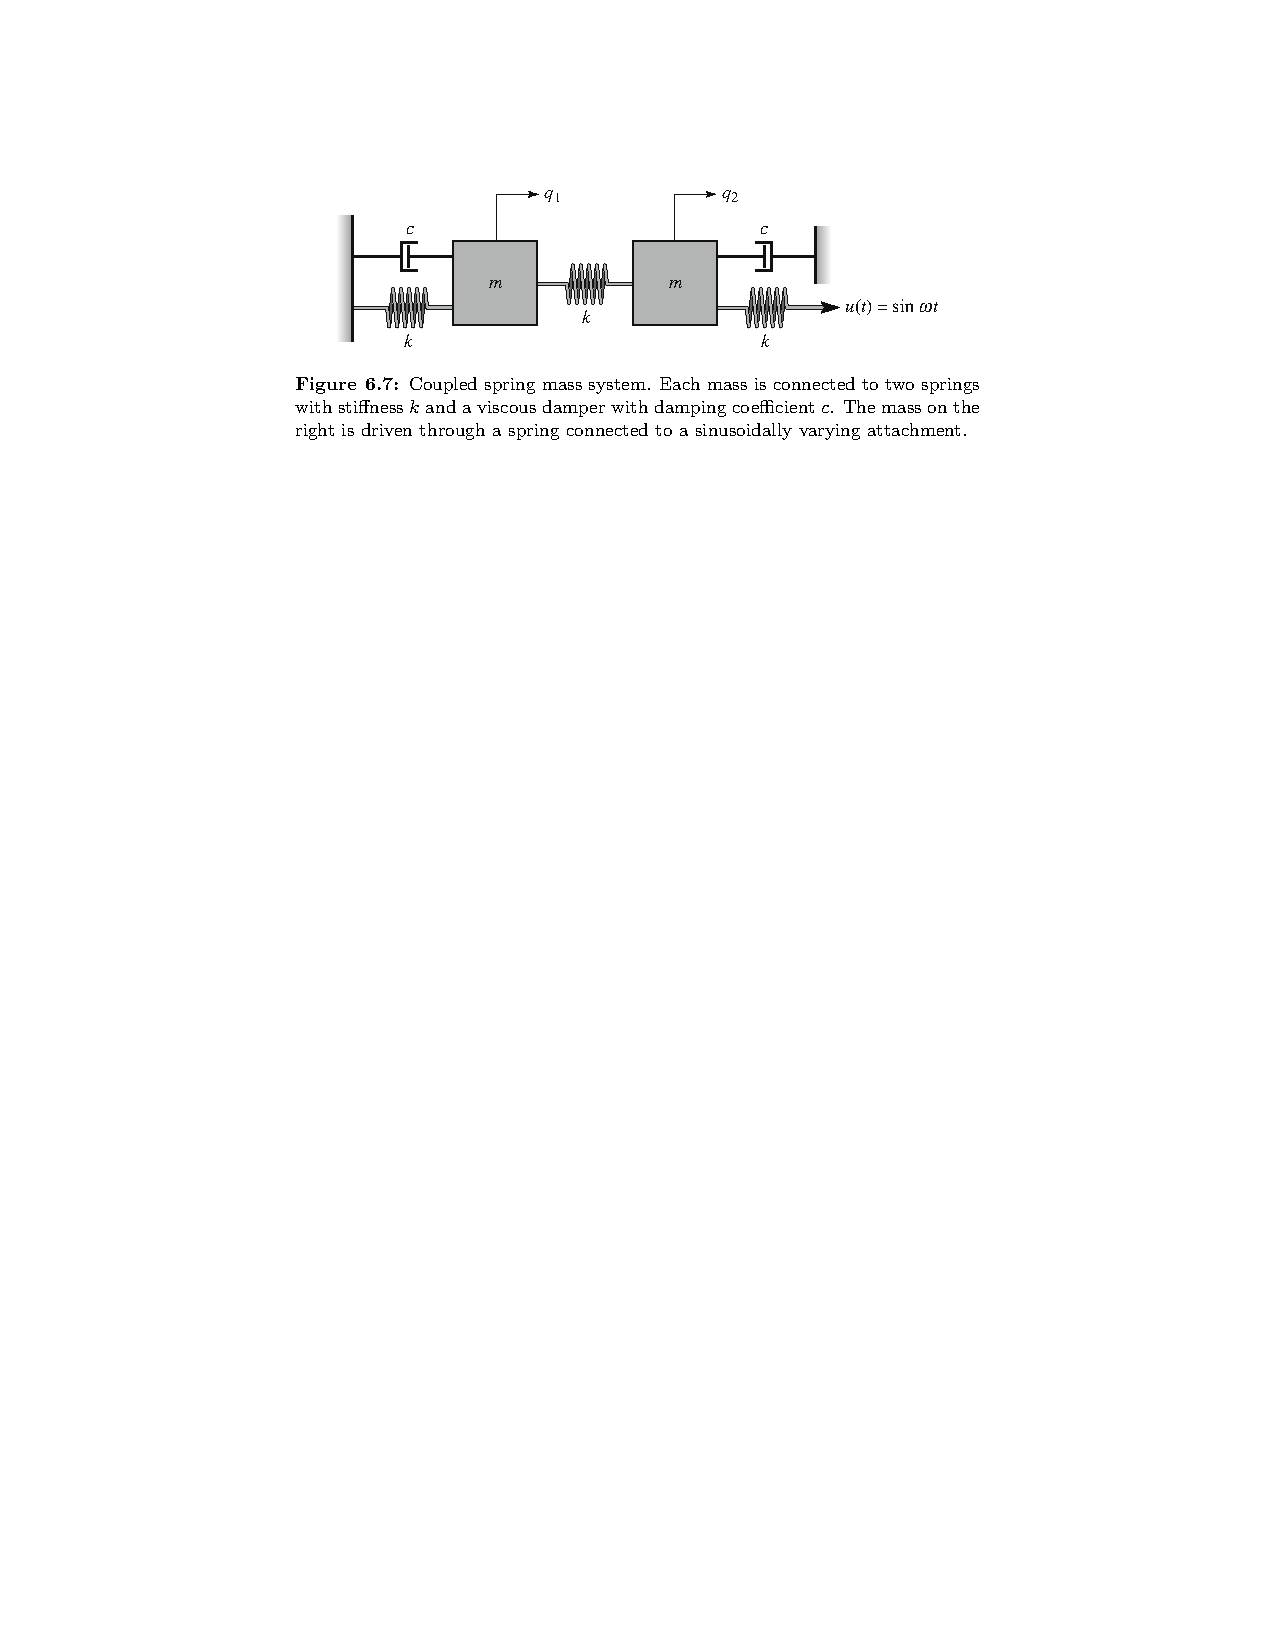
\includegraphics[width=\linewidth]{figure6.7}

\end{frame}

\begin{frame}
\frametitle{Coupled dynamics}

Original:
\[
\Deriv{}{t}\Matr{q_1\\q_2\\\dot q_1\\\dot q_2} =
\underbrace{\begin{bmatrix}
0 & 0 & 1 & 0 \\
0 & 0 & 0 & 1 \\
-\frac{2k}{m} & \frac{k}{m} & -\frac{c}{m} & 0 \\
\frac{k}{m} & -\frac{2k}{m} & 0 & -\frac{c}{m}
\end{bmatrix}}_{A}
\Matr{q_1\\q_2\\\dot q_1\\\dot q_2} +
\begin{bmatrix}
0 \\
0 \\
0 \\
\frac{k}{m}
\end{bmatrix}
u
\]
Transformation:
\[
z = T x = \frac{1}{2}
\begin{bmatrix}
1 & 1 & 0 & 0 \\
0 & 0 & 1 & 1 \\
1 & -1 & 0 & 0 \\
0 & 0 & 1 & -1
\end{bmatrix}
x
=
\frac12
\begin{bmatrix}
q_1 + q_2 \\
\dot{q}_1 + \dot{q}_2 \\
q_1 - q_2 \\
\dot{q}_1 - \dot{q}_2
\end{bmatrix}
\]


\end{frame}

\begin{frame}
\frametitle{Coupled dynamics}
Transformed:
\[
\Deriv{z}{t} =
\begin{bmatrix}
0 & 1 & 0 & 0 \\
-\frac{k}{m} & -\frac{c}{m} & 0 & 0 \\
0 & 0 & 0 & 1 \\
0 & 0 & -\frac{3k}{m} & -\frac{c}{m}
\end{bmatrix}
z +
\begin{bmatrix}
0 \\
\frac{k}{2m} \\
0 \\
-\frac{k}{2m}
\end{bmatrix}
u
\]
\begin{align}
\tilde A &= TAT^{-1} = 
\begin{bmatrix}
0 & 1 & 0 & 0 \\
-\frac{k}{m} & -\frac{c}{m} & 0 & 0 \\
0 & 0 & 0 & 1 \\
0 & 0 & -\frac{3k}{m} & -\frac{c}{m}
\end{bmatrix}
=
\begin{bmatrix}
\tilde A_1 & 0 \\
0 & \tilde A_2
\end{bmatrix}
\end{align}
\begin{itemize}
\item Confirm $A$, $\tilde A$, $\tilde A_1$, $\tilde A_2$ all have same eigenvalues
\end{itemize}

\end{frame}

\SUBCONCEPT{Steady-State Response}

\begin{frame}
\frametitle{Response}

\begin{tabular}{|p{2cm}|p{2cm}|p{2cm}|p{2cm}|}
\hline
\multicolumn{4}{|c|}{Response}\\
\hline
\multicolumn{2}{|c|}{Initial condition} & \multicolumn{2}{c|}{Forced}\\
\hline
 &  & Transient & Steady state\\
\hline
\end{tabular}
\bigskip

\begin{itemize}
\item
Transient response: from `mismatch' between initial condition and steady state
\item
Steady state: the long term trend
\end{itemize}
\bigskip

Usually steady-state characteristics follow the input (e.g. constant input leads to constant steady state)

\end{frame}

\begin{frame}
\frametitle{Transient vs steady state response}
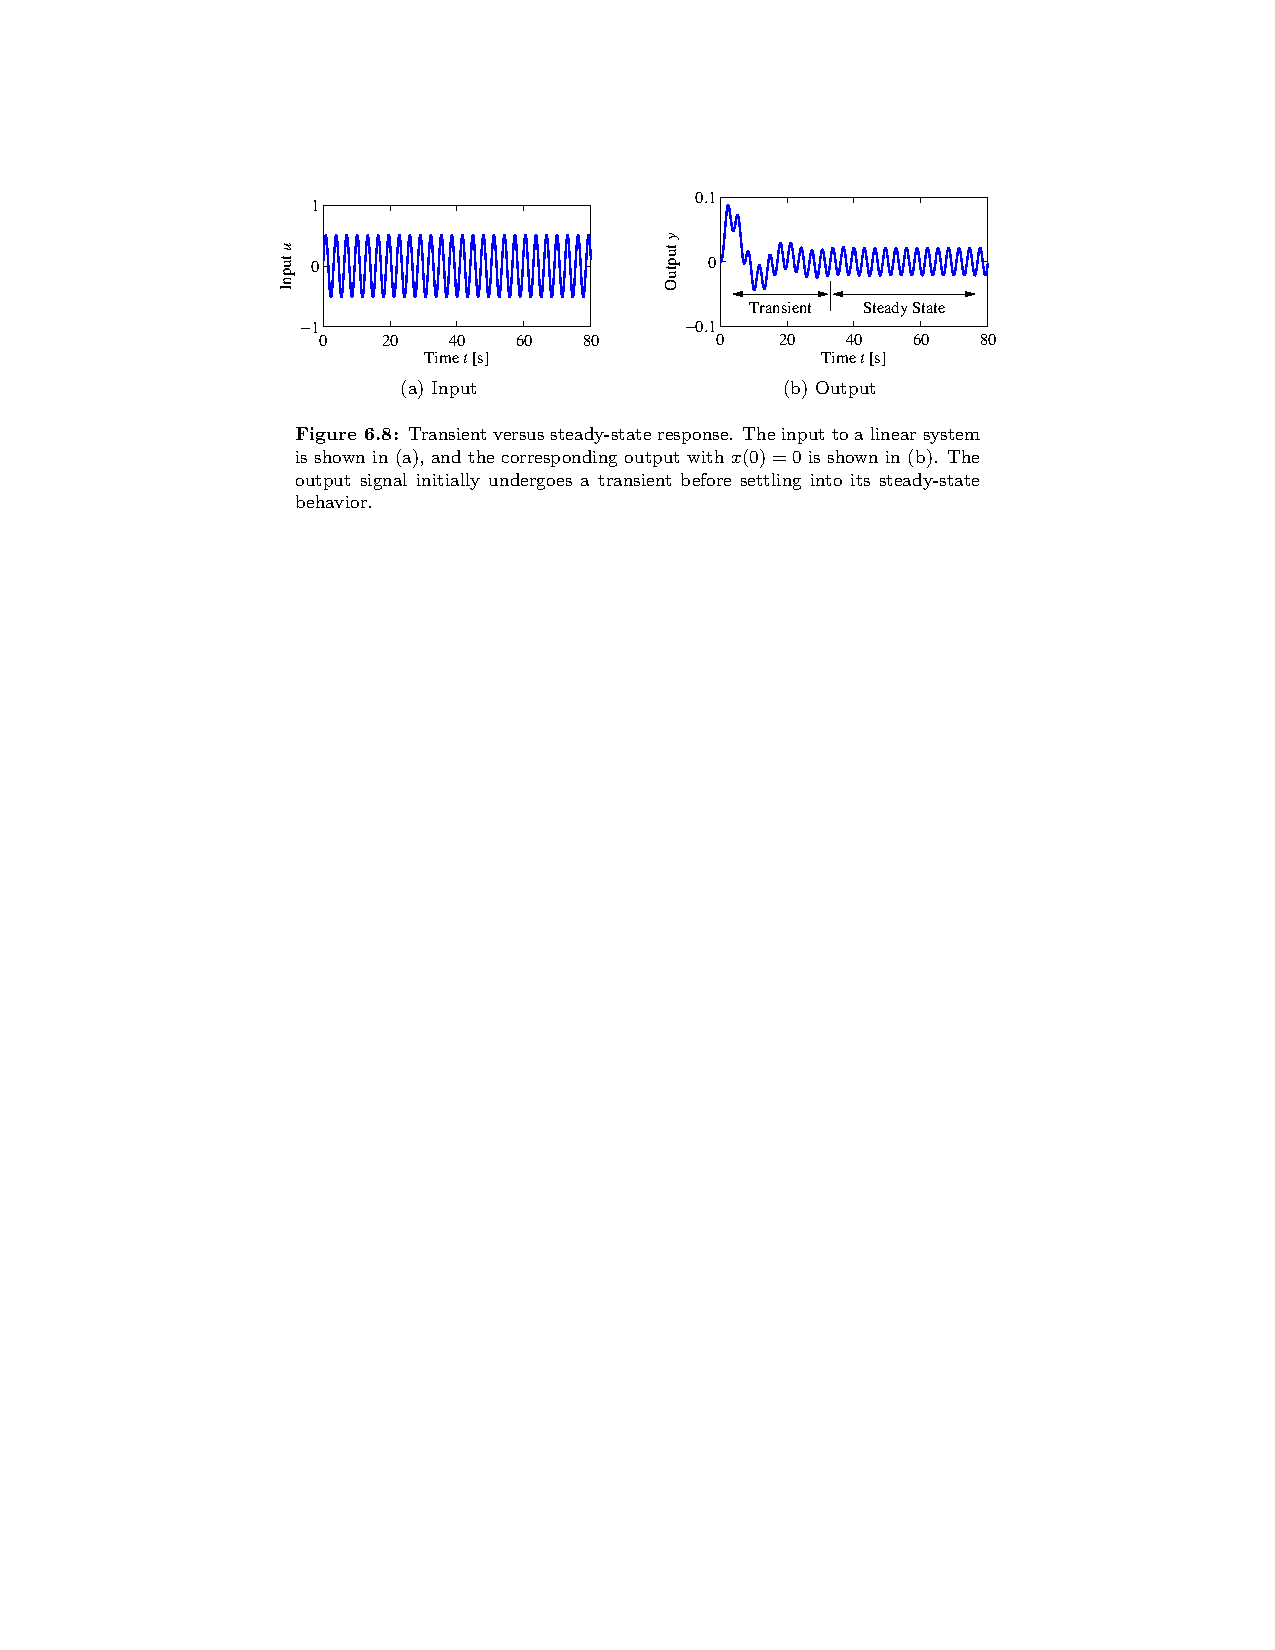
\includegraphics[width=\linewidth]{figure6.8}
\end{frame}

\begin{frame}
\frametitle{Step response}
\begin{align}
u(t) &= \StepInput(t)\,, & y(t) &= \StepResponse(t) = \underbrace{CA^{-1} \ee^{At} B}_{\text{transient}} + \underbrace{D-CA^{-1}B}_{\text{steady-state}}
\end{align}

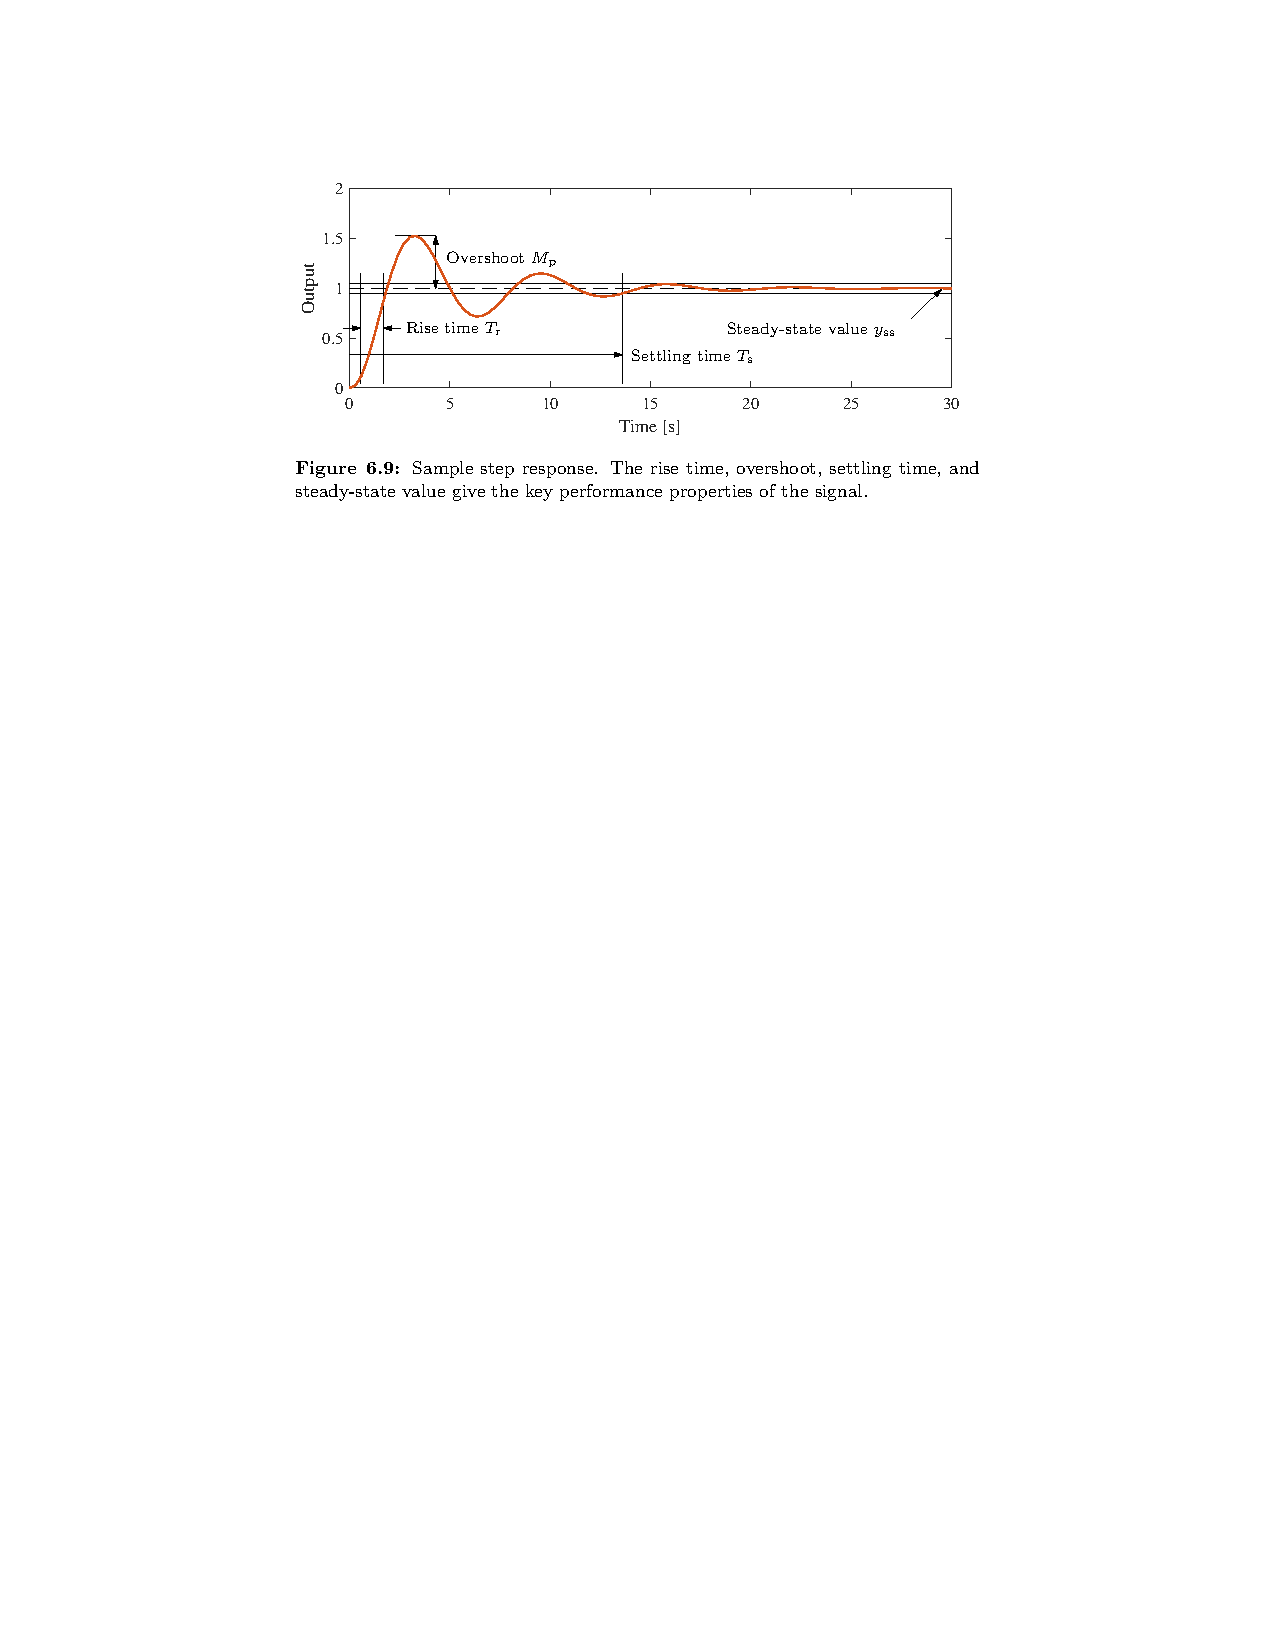
\includegraphics[width=\linewidth]{figure6.9}

\end{frame}


\SUBCONCEPT{Frequency Response}

\begin{frame}
\frametitle{Sinusoidal input}

\begin{align}
u(t) &= \ee^{st}, \qquad s=\ii\ww\,,\\
y(t) &= \underbrace{C \ee^{At} \left( x(0)-(sI-A)^{-1}B \right)}_{\text{transient}} + \underbrace{\left(C(sI-A)^{-1}B+D\right)\ee^{st}}_{\text{steady-state}} & 
\end{align}
Consider just steady-state:
\begin{align}
y_{ss}(t) &= \left(C(sI-A)^{-1}B+D\right)\ee^{st} \\
        &= G(s) \ee^{st}
\end{align}
For real sinusoidal input, 
\begin{align}
  u(t)&=\cos\ww t \,, &  y_{ss}(t)&= M \cos(\ww t + \theta)
\end{align}
where $M$ is gain and $\theta$ is phase:
\begin{align}
M &= |G(\ii w)| \,, & \theta &= \arg G(\ii w)
\end{align}

\end{frame}

\begin{frame}
\frametitle{Frequency response}
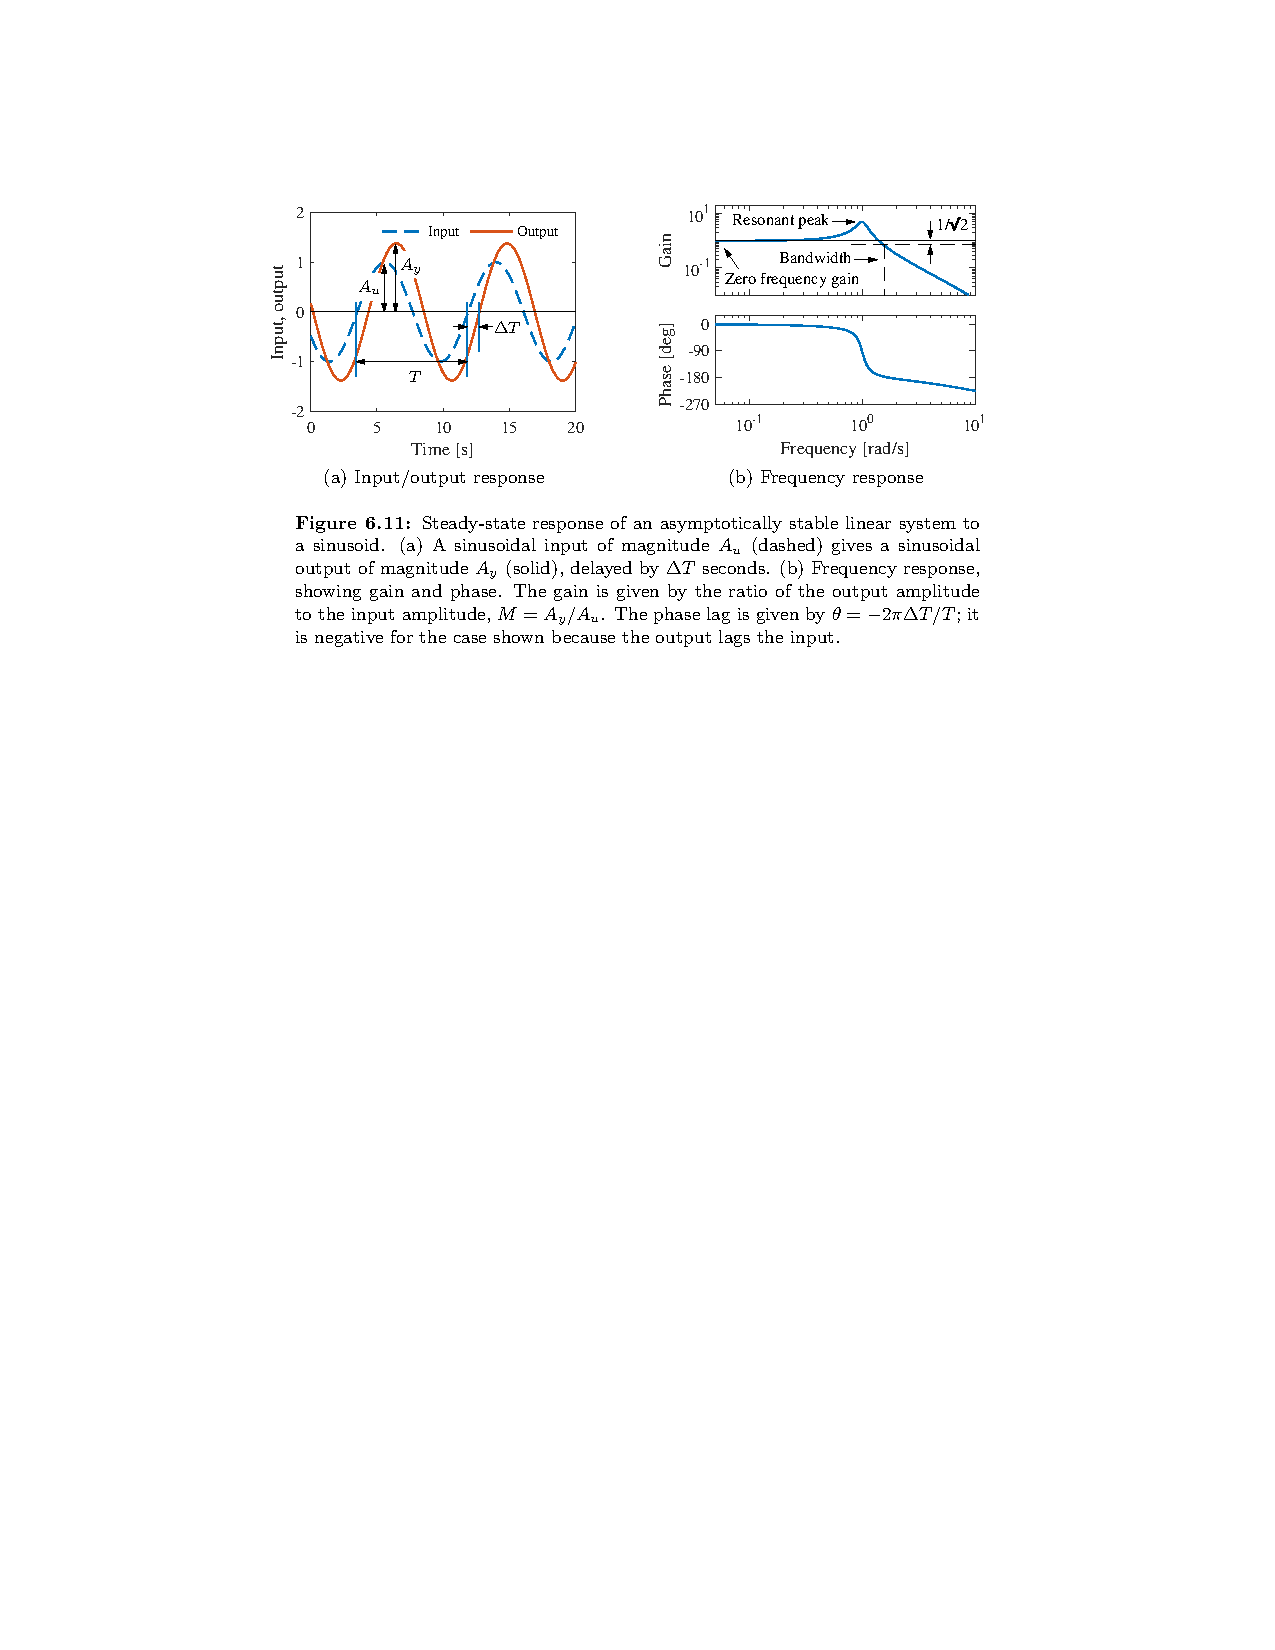
\includegraphics[width=\linewidth]{figure6.11}
\end{frame}

\begin{frame}
\frametitle{Frequency response characteristics}
\begin{description}
\item[Zero frequency gain, $\DCgain$] ~\\Gain for constant inputs (i.e., zero frequency): \[\DCgain = \lim_{\ww\to0}|G(\ii\ww)| = -CA^{-1}B+D\]
\item[Bandwidth, $\wb$] ~\\Frequency range above $\sqrt{\frac12}$ of `reference' (zero frequency gain, usually)
\item[Resonance peak $\Mpeak$ and peak frequency $\wres$] ~\\Maximum amplitude of frequency response gain, and corresponding frequency at which this occurs
\end{description}
\end{frame}

\SUMMARYFRAME
\FINALE

\end{document}
